\documentclass[ucs,9pt]{beamer}

% Copyright 2004 by Till Tantau <tantau@users.sourceforge.net>.
%
% In principle, this file can be redistributed and/or modified under
% the terms of the GNU Public License, version 2.
%
% However, this file is supposed to be a template to be modified
% for your own needs. For this reason, if you use this file as a
% template and not specifically distribute it as part of a another
% package/program, I grant the extra permission to freely copy and
% modify this file as you see fit and even to delete this copyright
% notice.
%
% Modified by Tobias G. Pfeiffer <tobias.pfeiffer@math.fu-berlin.de>
% to show usage of some features specific to the FU Berlin template.

% remove this line and the "ucs" option to the documentclass when your editor is not utf8-capable
\usepackage[utf8x]{inputenc}    % to make utf-8 input possible
\usepackage[german]{babel}     % hyphenation etc., alternatively use 'german' as parameter
\usepackage[inkscape={/usr/bin/inkscap‌​e -z -C}]{svg}
\usepackage{amsmath}
% Template for talks using the Corporate Design of the Freie Universitaet
%   Berlin, created following the guidelines on www.fu-berlin.de/cd by
%   Tobias G. Pfeiffer, <tobias.pfeiffer@math.fu-berlin.de>
% This file can be redistributed and/or modified in any way you like.
%   If you feel you have done significant improvements to this template,
%   please consider providing your modified version to
%   https://www.mi.fu-berlin.de/w/Mi/BeamerTemplateCorporateDesign

\usepackage{amsmath,dsfont,listings}

%%% FU logo
% small version for upper right corner of normal pages
\pgfdeclareimage[height=0.9cm]{university-logo}{FULogo_RGB}
\logo{\pgfuseimage{university-logo}}
% large version for upper right corner of title page
\pgfdeclareimage[height=1.085cm]{big-university-logo}{FULogo_RGB}
\newcommand{\titleimage}[1]{\pgfdeclareimage[height=2.92cm]{title-image}{#1}}
\titlegraphic{\pgfuseimage{title-image}}
%%% end FU logo

% NOTE: 1cm = 0.393 in = 28.346 pt;    1 pt = 1/72 in = 0.0352 cm
\setbeamersize{text margin right=3.5mm, text margin left=7.5mm}  % text margin

% colors to be used
\definecolor{text-grey}{rgb}{0.45, 0.45, 0.45} % grey text on white background
\definecolor{bg-grey}{rgb}{0.66, 0.65, 0.60} % grey background (for white text)
\definecolor{fu-blue}{RGB}{0, 51, 102} % blue text
\definecolor{fu-green}{RGB}{153, 204, 0} % green text
\definecolor{fu-red}{RGB}{204, 0, 0} % red text (used by \alert)

% switch off the sidebars
% TODO: loading \useoutertheme{sidebar} (which is maybe wanted) also inserts
%   a sidebar on title page (unwanted), also indents the page title (unwanted?),
%   and duplicates the navigation symbols (unwanted)
\setbeamersize{sidebar width left=0cm, sidebar width right=0mm}
\setbeamertemplate{sidebar right}{}
\setbeamertemplate{sidebar left}{}
%    XOR
% \useoutertheme{sidebar}

% frame title
% is truncated before logo and splits on two lines
% if neccessary (or manually using \\)
\setbeamertemplate{frametitle}{%
    \vskip-30pt \color{text-grey}\large%
    \begin{minipage}[b][23pt]{80.5mm}%
    \flushleft\insertframetitle%
    \end{minipage}%
}

%%% title page
% TODO: get rid of the navigation symbols on the title page.
%   actually, \frame[plain] *should* remove them...
\setbeamertemplate{title page}{
% upper right: FU logo
\vskip2pt\hfill\pgfuseimage{big-university-logo} \\
\vskip6pt\hskip3pt
% title image of the presentation
\begin{minipage}{11.6cm}
\hspace{-1mm}\inserttitlegraphic
\end{minipage}

% set the title and the author
\vskip14pt
\parbox[top][1.35cm][c]{11cm}{\color{text-grey}\inserttitle \\ \small \insertsubtitle}
\vskip11pt
\parbox[top][1.35cm][c]{11cm}{\small \insertauthor \\ \insertinstitute \\[3mm] \insertdate}
}
%%% end title page

%%% colors
\usecolortheme{lily}
\setbeamercolor*{normal text}{fg=black,bg=white}
\setbeamercolor*{alerted text}{fg=fu-red}
\setbeamercolor*{example text}{fg=fu-green}
\setbeamercolor*{structure}{fg=fu-blue}

\setbeamercolor*{block title}{fg=white,bg=black!50}
\setbeamercolor*{block title alerted}{fg=white,bg=black!50}
\setbeamercolor*{block title example}{fg=white,bg=black!50}

\setbeamercolor*{block body}{bg=black!10}
\setbeamercolor*{block body alerted}{bg=black!10}
\setbeamercolor*{block body example}{bg=black!10}

\setbeamercolor{bibliography entry author}{fg=fu-blue}
% TODO: this doesn't work at all:
\setbeamercolor{bibliography entry journal}{fg=text-grey}

\setbeamercolor{item}{fg=fu-blue}
\setbeamercolor{navigation symbols}{fg=text-grey,bg=bg-grey}
%%% end colors

%%% headline
\setbeamertemplate{headline}{
\vskip4pt\hfill\insertlogo\hspace{3.5mm} % logo on the right

\vskip6pt\color{fu-blue}\rule{\textwidth}{0.4pt} % horizontal line
}
%%% end headline

%%% footline
\newcommand{\footlinetext}{\insertshortinstitute, \insertshorttitle, \insertshortdate}
\setbeamertemplate{footline}{
\vskip5pt\color{fu-blue}\rule{\textwidth}{0.4pt}\\ % horizontal line
\vskip2pt
\makebox[123mm]{\hspace{7.5mm}
\color{fu-blue}\footlinetext
\hfill \raisebox{-1pt}{\usebeamertemplate***{navigation symbols}}
\hfill \insertframenumber}
\vskip4pt
}
%%% end footline

%%% settings for listings package
\lstset{extendedchars=true, showstringspaces=false, basicstyle=\footnotesize\sffamily, tabsize=2, breaklines=true, breakindent=10pt, frame=l, columns=fullflexible}
\lstset{language=Java} % this sets the syntax highlighting
\lstset{mathescape=true} % this switches on $...$ substitution in code
% enables UTF-8 in source code:
\lstset{literate={ä}{{\"a}}1 {ö}{{\"o}}1 {ü}{{\"u}}1 {Ä}{{\"A}}1 {Ö}{{\"O}}1 {Ü}{{\"U}}1 {ß}{\ss}1}
%%% end listings  % THIS is the line that includes the FU template!
\setbeamertemplate{navigation symbols}{} 
\usepackage{arev,t1enc} % looks nicer than the standard sans-serif font
% if you experience problems, comment out the line above and change
% the documentclass option "9pt" to "10pt"

% image to be shown on the title page (without file extension, should be pdf or png)
\titleimage{linux-logo}

\title[Linux - Access Control] % (optional, use only with long paper titles)
{Linux - Access Control}

\subtitle
{}

\author[Author, Another] % (optional, use only with lots of authors)
{Martin Görick, Dennis Hägler und Kai Kriedemann}
% - Give the names in the same order as the appear in the paper.

\institute[FU Berlin] % (optional, but mostly needed)
{Freie Universität Berlin}
% - Keep it simple, no one is interested in your street address.

\date[] % (optional, should be abbreviation of conference name)
{Rechersicherheit}
% - Either use conference name or its abbreviation.
% - Not really informative to the audience, more for people (including
%   yourself) who are reading the slides online

\subject{}
% This is only inserted into the PDF information catalog. Can be left
% out.

% you can redefine the text shown in the footline. use a combination of
% \insertshortauthor, \insertshortinstitute, \insertshorttitle, \insertshortdate, ...
\renewcommand{\footlinetext}{\insertshortinstitute, \insertshorttitle, \insertshortdate}

% Delete this, if you do not want the table of contents to pop up at
% the beginning of each subsection:
%\AtBeginSection[]
%{
%  \begin{frame}<beamer>{Outline}
%    \tableofcontents[currentsection,hideothersubsections]
%  \end{frame}
%}

\begin{document}

\begin{frame}[plain]
  \titlepage
\end{frame}

\begin{frame}{Outline}
  \tableofcontents[hideothersubsections]
  % You might wish to add the option [pausesections]
\end{frame}

%\section{Introduction}

%\begin{frame}{title of frame} %title in brace
%\begin{itemize}
%\item test item
%\end{itemize}
%\end{frame}

\section{Zugriffsrechte}

\begin{frame}{Zugriffsrechte}
\begin{itemize}
	\item lesen/ read
		\begin{itemize}
			\item erlaubt lesen einer Datei
			\item abrufen von enthaltene Dateien
		\end{itemize}
	\item schreiben/ write
		\begin{itemize}
			\item erlaubt beschreiben einer Datei
			\item erstellen oder löschen von Dateien
			\item Eigenschaften enthaltener Dateien verändern 
		\end{itemize}
	\item ausführen/ execute
		\begin{itemize}
			\item ausführen von Dateien erlaubt
			\item recht in ein Verzeichnis zu wechseln
			\item Attribute von Dateien abrufen
		\end{itemize}
\end{itemize}
\end{frame}

\begin{frame}{Zugriffsrechte ändern und setzen}
\begin{itemize}
	\item möglich nur mit root rechten
	\item chgrp - Gruppe ändern 
	\item chown - Besitzer oder/ und Gruppe ändern
	\item chmod - Rechte ändern
\end{itemize}
\end{frame}

\section{Benutzergruppen, Protection Rings}

\subsection{Benutzergruppen}

\begin{frame}{Benutzergruppen}
\begin{itemize}
\item jeder Benutzer in einer Hauptgruppe
\item kann in beliebigen anderen Gruppen sein
\item Hardwarezugriff auf Gruppen beschränkt
\item jede Datei ist Eigentums eines Benutzers
\item jede Datei ist einer Gruppe zugeordnet
\item Datei erstellen $\rightarrow$ Hauptgruppe des Erstellers
\end{itemize}
\end{frame}

\begin{frame}{Namenskonventionen}
\begin{itemize}
\item beginnen mit Kleinbuchstaben
\item gefolgt von a-z, -, \_
\item möglich am Ende des Namen \$ (Kompatibilität Samba-Rechner)
\item einzigartig
\end{itemize}
\begin{itemize}
\item Regeln festgelegt in /etc/adduser.conf
\end{itemize}
\end{frame}

\begin{frame}{Protection Rings}
\begin{figure}
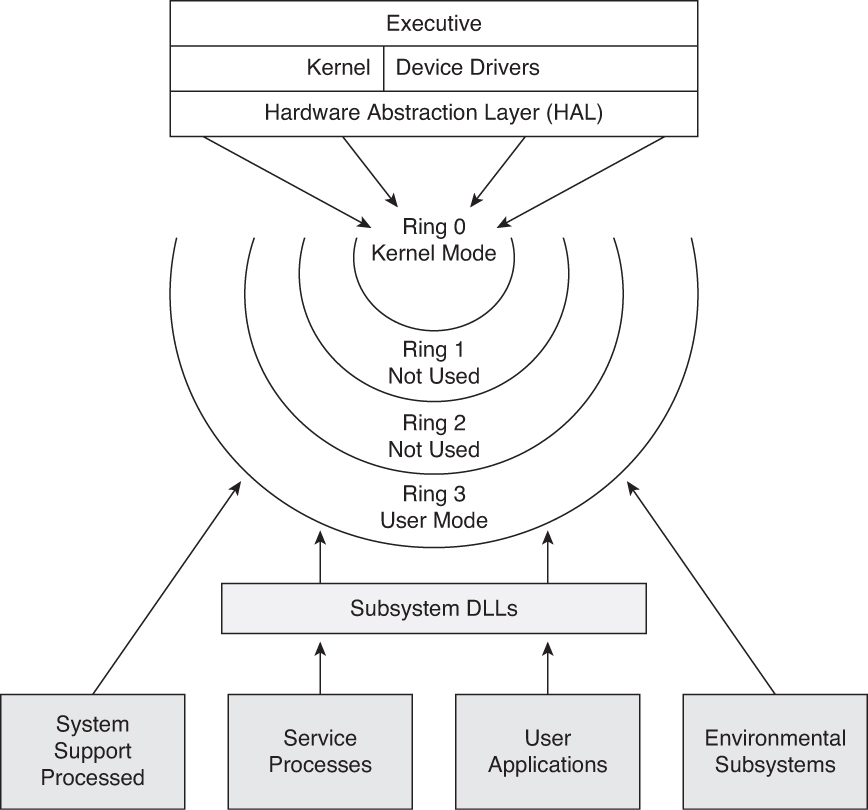
\includegraphics[scale=0.3]{protectionRings}
\caption{Quelle \url{http://ptgmedia.pearsoncmg.com/images/chap5_9780789749574/elementLinks/05fig04_alt.jpg}}
\end{figure}
\end{frame}

\section{Zugriffsmatrix Realisation}

\begin{frame}{Zugriffsmatrix Realisation}
\begin{itemize}
\item Zugriffslisten ACL
\item Access ACL
	\begin{itemize}
		\item Zugriffsrecht von Gruppen und Benutzern auf beliebige Dateisystemobjekte
	\end{itemize}
\item Default ACL
	\begin{itemize}
		\item nur auf Verzeichnisse
		\item welche Recht vom übergeordneten Verzeichnis geerbt
	\end{itemize}
\item ACL Eintrag
	\begin{itemize}
		\item minimal - owner, group, other
		\item erweitert - mask-Eintrag, named users, named groups
	\end{itemize}
\end{itemize}
\end{frame}

\section{Zugriffsmatrix Schutz (Reference Monitor)}

\begin{frame}{Zugriffsmatrix Schutz (Reference Monitor)}
\begin{itemize}
\item LSM - Framework und Schnittstelle für Reference Monitor
\item Implementierung im SELinux
\item vorgehen:
	\begin{itemize}
		\item LSM hooks via Systemaufrufe
		\item hook besitzt Referenz auf Linux Objekte
		\item in konforme Authorisierungsqueries transformieren
		\item Authorisierungsqueries für Protektion System verarbeitet
	\end{itemize}
\end{itemize}
\end{frame}

%\begin{frame}[fragile]
%  \frametitle{Test code frame}
%\begin{semiverbatim}
%Testcode
%\end{semiverbatim}
%\end{frame}

%\section{Test Section 2}

%\begin{frame}{}
%\begin{figure}
%
\includegraphics[scale=0.5]{linux-logo}
%\caption{linux-logo}
%\end{figure}
%\end{frame}



% All of the following is optional and typically not needed. 
\appendix
\section<presentation>*{\appendixname}
\subsection<presentation>*{For Further Reading}

\begin{frame}[allowframebreaks]
  \frametitle<presentation>{For Further Reading}
    
  \begin{thebibliography}{10}

  \beamertemplatearticlebibitems
  % Followed by interesting articles. Keep the list short. 

  \bibitem{PR}
    Protection Ring Picture
    \newblock \url{http://ptgmedia.pearsoncmg.com/images/chap5_9780789749574/elementLinks/05fig04_alt.jpg}
  \bibitem{ACL}
    Access Control Lists unter Linux
    \newblock \url{http://users.suse.com/~agruen/acl/chapter/fs_acl-de.pdf}  
  \bibitem{LSM}
    Case Study: Building a Secure Operating System for Linux
    \newblock \url{http://www.cse.psu.edu/~trj1/cse443-s12/docs/ch9.pdf}  
  \end{thebibliography}
\end{frame}


\end{document}
